\documentclass[journal]{IEEEtran}

\usepackage{cite}
\usepackage{amsmath,amssymb,amsfonts}
\usepackage{graphicx}
\usepackage{textcomp}
\usepackage{xcolor}
\usepackage{booktabs}
\usepackage{array}
\usepackage{url}
\usepackage[caption=false,font=footnotesize]{subfig}
\graphicspath{{figs/}}

\def\BibTeX{{\rm B\kern-.05em{\sc i\kern-.025em b}\kern-.08em
    T\kern-.1667em\lower.7ex\hbox{E}\kern-.125emX}}

\begin{document}

\title{ASCEND: An Autonomous Aerial Surveyor for\\
GNSS-Denied Exploration, Mapping, Feature\\
Identification, and Precision Self-Docking}

\author{Robotech,~\IEEEmembership{National Institute of Technology Karnataka}%
\thanks{Manuscript prepared April~2026. This work was carried out for the
ISRO Robotics Challenge--Unmanned (IRoC-U) 2026, Team ID~11108.}%
\thanks{The authors are with the Department of Engineering,
National Institute of Technology Karnataka, Surathkal, India.}}

\markboth{Design and Development of an Autonomous Aerial Surveyor (ASCEND), IRoC-U 2026}%
{Robotech NITK: ASCEND --- Autonomous Aerial Surveyor for GNSS-Denied Operation}

\maketitle

\begin{abstract}
Autonomous aerial operation in GNSS-denied environments demands a tightly
integrated stack spanning closed-loop flight stabilization, drift-bounded
state estimation, online mapping, semantic feature identification, and
reliable physical recovery. This paper presents \emph{ASCEND}
(Autonomous Surveyor Challenge for Exploration, Navigation and Dynamics),
a quadrotor--base-station system that unifies deployment, exploration,
feature documentation, and self-recovery into a single mission framework
that requires no human intervention or external positioning aids.
The vehicle estimates its pose using a two-tier scheme that fuses
camera-based optical flow and visual--inertial odometry at high rate with
a lower-rate 2D-LiDAR SLAM backend that bounds drift and builds a globally
consistent occupancy grid. Cascaded attitude, altitude, and position
control loops---running on an ArduPilot flight controller and reconfigured
to consume optical-flow and rangefinder measurements through EKF3---provide
centimeter-level station keeping without GNSS. Targets of interest are
detected onboard with a lightweight vision pipeline and validated at the
base station against seed imagery using SIFT features, FLANN matching with
Lowe's ratio test, and RANSAC homography estimation. Recovery is achieved
through a vision- and LiDAR-guided precision docking sequence onto a
funnel-shaped (frustum) charging platform, where an HSV color-masking and
shape-classification pipeline localizes the pad and a Hough-circle--based
2D-LiDAR controller centers the vehicle for touchdown and automatic
magnetic charging. We describe the complete mechanical, electrical, and
software design, the hardware selection rationale, the power and mass
budget, and the emergency-response architecture. The resulting platform
establishes a reproducible and scalable foundation for autonomous aerial
survey missions.
\end{abstract}

\begin{IEEEkeywords}
Autonomous UAV, GNSS-denied navigation, optical flow, visual--inertial
odometry, 2D LiDAR SLAM, frontier exploration, precision docking, SIFT,
RANSAC, ArduPilot, ROS~2.
\end{IEEEkeywords}

\section{Introduction}
\IEEEPARstart{A}{utonomous} aerial vehicles are increasingly tasked with
surveying environments where the Global Navigation Satellite System (GNSS)
is unavailable or unreliable---indoor structures, dense terrain, planetary
analogues, and disaster sites. In such settings the vehicle must localize,
map, and make navigation decisions using only onboard sensing, while still
guaranteeing safe recovery at the end of a mission. \emph{ASCEND} is an
autonomous aerial system designed to meet exactly these requirements. It
integrates deployment, exploration, feature identification, and recovery
into a single closed framework.

The system comprises a micro-UAV and a base station. The UAV acquires
reference (``seed'') data, explores unknown areas, documents features of
interest, and then returns to the base station for data validation
without any human intervention or external navigation aids. Autonomy is
driven by layered sensing and control: closed-loop flight stabilization
ensures reliable maneuvering, while onboard LiDAR and vision sensors
estimate the UAV's pose relative to the base station. The UAV maps its
surroundings in real time to support obstacle avoidance and path planning,
and onboard decision logic enables navigation without prior maps, adapting
trajectories to environmental constraints.

A quadcopter platform was selected for its high positional control and
mechanical simplicity. This configuration provides sufficient payload
capacity and balanced thrust distribution while maintaining unobstructed
sensor placement. By prioritizing the perception and navigation challenges
relevant to future survey operations, ASCEND establishes a scalable
foundation for autonomous aerial exploration and repeatable mission
execution. The end-to-end data flow of the system is summarized in
Fig.~\ref{fig:block}, and the assembled vehicle is shown in
Fig.~\ref{fig:vehicle}.

\begin{figure}[!t]
\centering
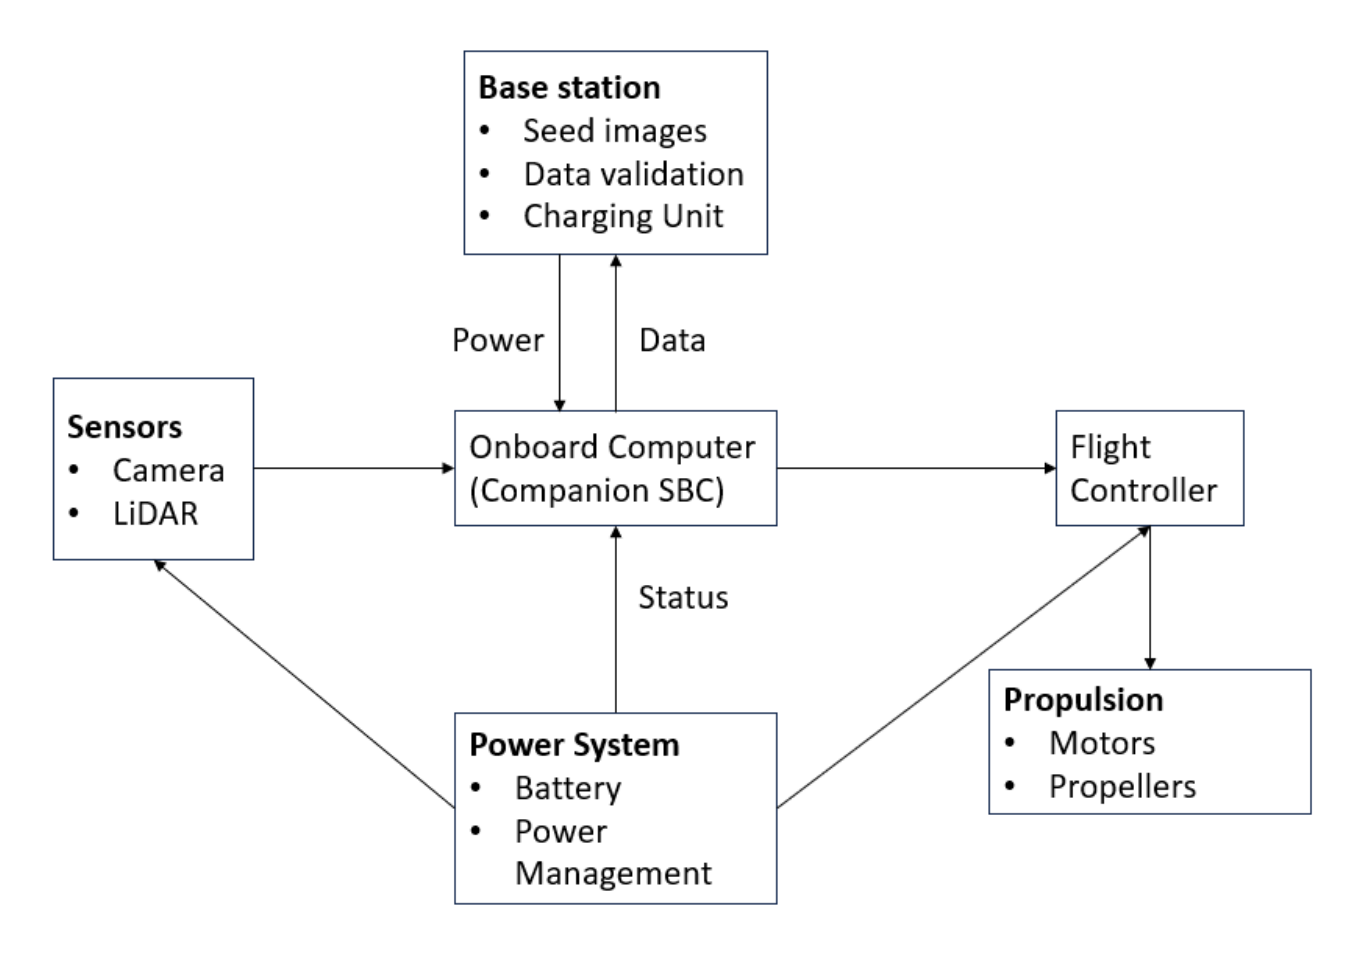
\includegraphics[width=\columnwidth]{fig01_block.png}
\caption{Block diagram of the ASCEND system, showing the flow of data
between sensing, estimation, control, mapping, perception, and the base
station.}
\label{fig:block}
\end{figure}

\begin{figure}[!t]
\centering
\subfloat[Front view]{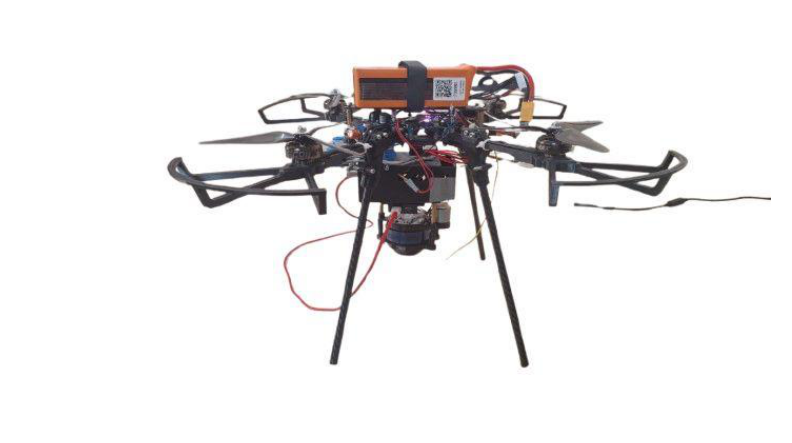
\includegraphics[width=0.52\columnwidth]{fig02a_front.png}}
\hfil
\subfloat[Top view]{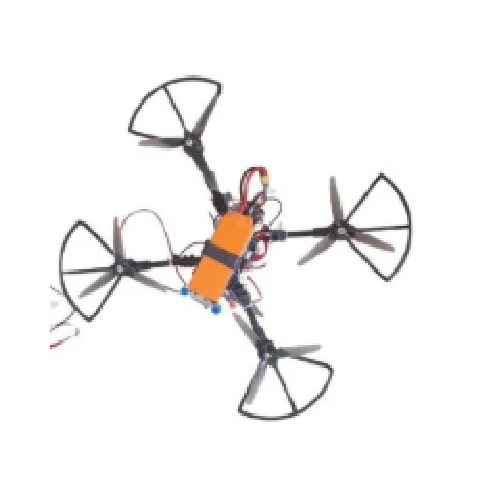
\includegraphics[width=0.40\columnwidth]{fig02b_top.png}}
\caption{The ASCEND quadrotor airframe with integrated downward LiDAR,
global-shutter camera, and companion computer.}
\label{fig:vehicle}
\end{figure}

The remainder of this paper is organized as follows.
Section~\ref{sec:mech} details the mechanical design, including the docking
frustum, base station, charging subsystem, airframe, and component mounts.
Section~\ref{sec:flight} describes the cascaded flight-control architecture.
Section~\ref{sec:nav} presents the GNSS-denied navigation stack, covering
two-tier estimation, SLAM, frontier exploration, and relocalization.
Section~\ref{sec:ml} describes the perception and validation pipeline.
Section~\ref{sec:state} formalizes the mission state machine and precision
docking. Section~\ref{sec:hw} reviews the hardware selection,
Section~\ref{sec:budget} the system and power budget,
Section~\ref{sec:safety} the emergency-response system, and
Section~\ref{sec:novelty} the principal novelties. Section~\ref{sec:concl}
concludes.

\section{Mechanical Design}
\label{sec:mech}

\subsection{Docking Frustum}
The terminal recovery phase relies on a passively self-aligning,
funnel-shaped (frustum) landing structure. During descent the UAV uses
optical flow and HSV masking to determine the landing area; the frustum
geometry then mechanically corrects residual lateral error, guiding the
vehicle to the geometric center for a high-precision touchdown. A
downward-facing 1D LiDAR continuously monitors altitude during descent.
Upon crossing a predefined altitude threshold (the frustum height), the 2D
LiDAR initiates a cross-sectional scan of the frustum and dynamically
guides the drone to the geometric center for precision touchdown.

The frustum geometry, summarized in Table~\ref{tab:frustum}, is driven by
the vehicle envelope. A mandatory $200$~mm radial clearance between the
propeller blades and the inner cone surface prevents mechanical
obstruction; given the drone dimensions and this clearance, the half-angle
of the cone is $50.6^{\circ}$. An outer diameter of $1370$~mm absorbs
landing inaccuracies observed during testing. The frustum is fabricated
from 18-gauge galvanized iron (GI), selected for its high rigidity-to-weight
ratio, and is reinforced by a modular aluminum-extrusion support framework
that suppresses wobble during docking and doubles as a protective housing
for the base-station power electronics (Figs.~\ref{fig:basestation}
and~\ref{fig:bs_views}).

\begin{table}[!t]
\centering
\caption{Frustum Geometry}
\label{tab:frustum}
\begin{tabular}{cccc}
\toprule
Half-angle ($^{\circ}$) & Outer dia.\ (mm) & Inner dia.\ (mm) & Height (mm)\\
\midrule
$50.67$ & $1370$ & $420$ & $390$\\
\bottomrule
\end{tabular}
\end{table}

\begin{figure}[!t]
\centering
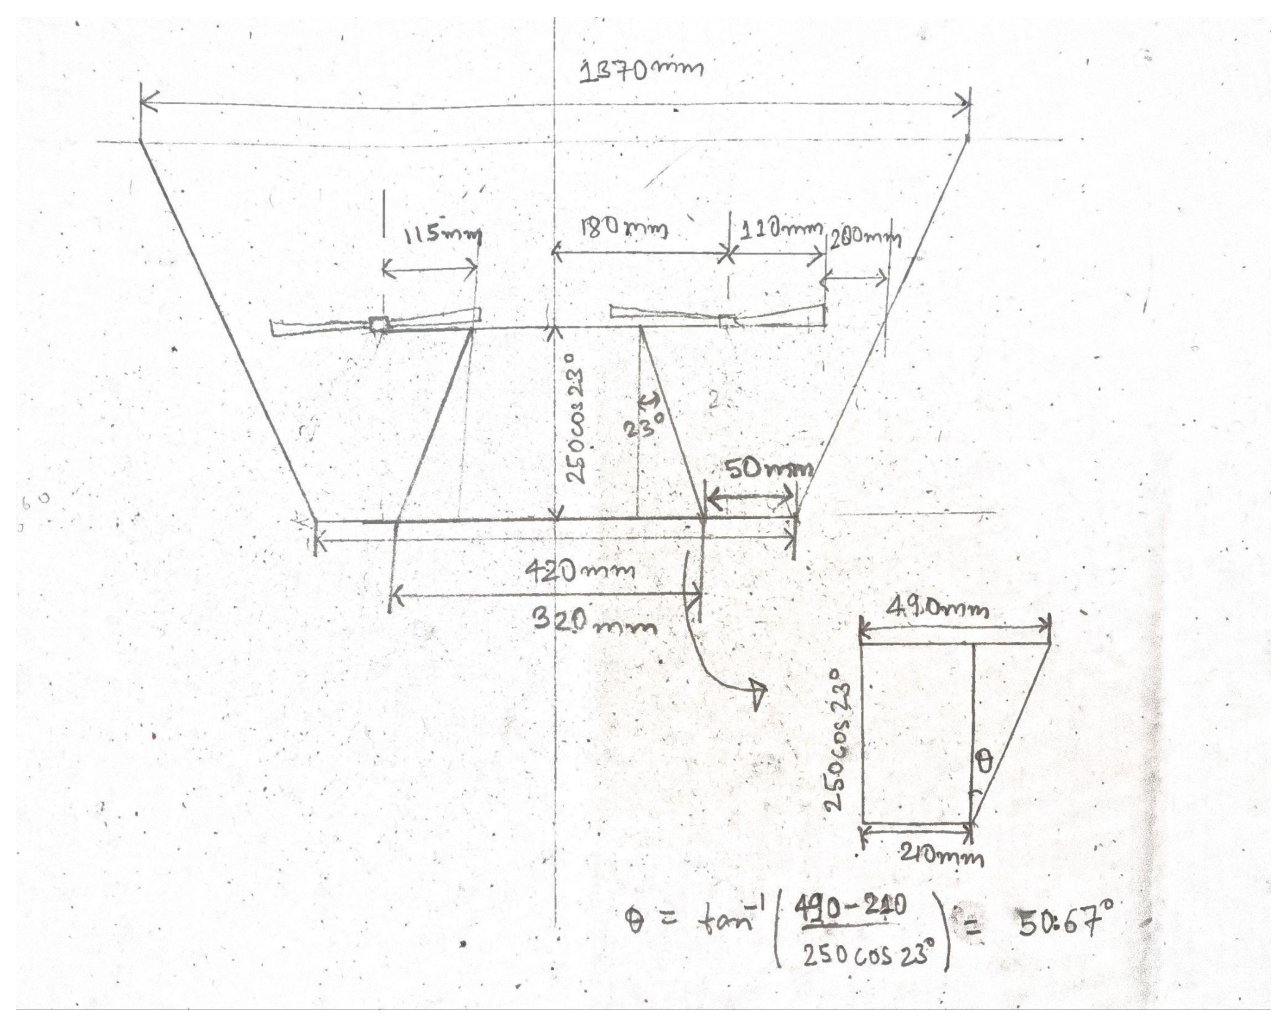
\includegraphics[width=0.78\columnwidth]{fig03_basestation.png}
\caption{Sketch of the base station with the self-aligning frustum and
modular support framework.}
\label{fig:basestation}
\end{figure}

\begin{figure}[!t]
\centering
\subfloat[Side view]{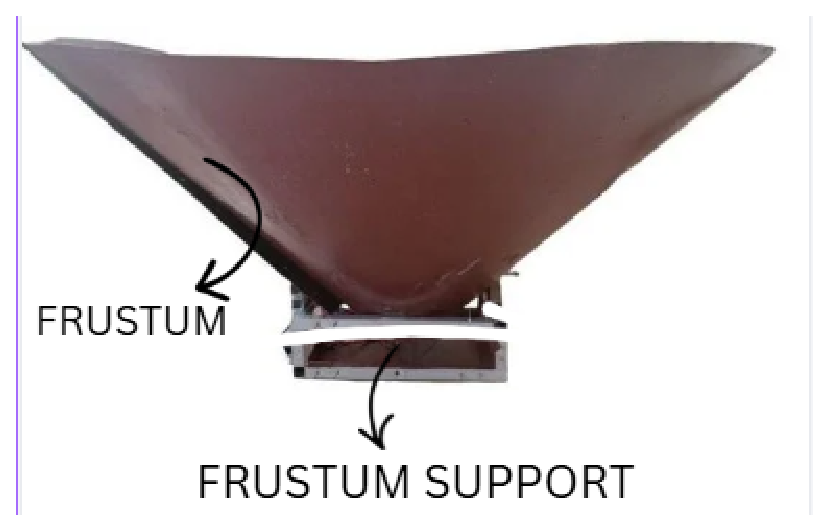
\includegraphics[width=0.46\columnwidth]{fig04a_side.png}}
\hfil
\subfloat[Top view]{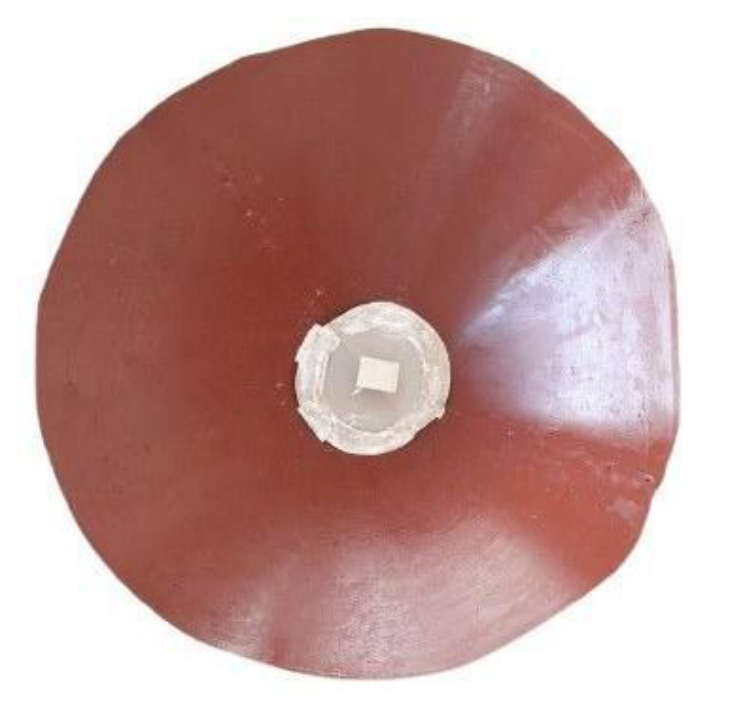
\includegraphics[width=0.40\columnwidth]{fig04b_top.png}}\\
\subfloat[Landing pad: spring-damped GI surface with magnetic charging
interface]{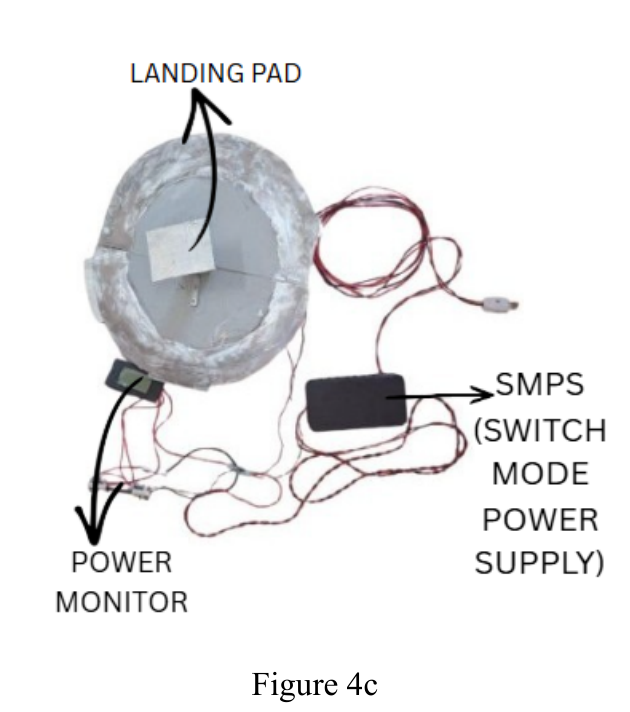
\includegraphics[width=0.55\columnwidth]{fig04c_pad.png}}
\caption{Base-station views. A circular GI sheet forms the touchdown zone;
an integrated spring mechanism (PVC- and clamp-supported) dampens landing
energy, and a magnetic coupling establishes the charging circuit.}
\label{fig:bs_views}
\end{figure}

\subsection{Charging Subsystem of the Base Station}
The terminal phase of the docking sequence physically mates the UAV with
the base station. The landing pad integrates a magnetic coupling that
aligns with copper charging plates on the UAV; on touchdown a closed
circuit is formed and charging begins automatically. The power electronics
convert standard grid AC into the regulated DC required to safely charge
the onboard 6S LiPo battery, while a display continuously monitors
electrical parameters and estimates the state of charge.

An AC--DC switch-mode power supply (SMPS, Fig.~\ref{fig:psu}) steps down and
rectifies the $100$--$240$\,V AC mains to a regulated $24$\,V DC output rated
up to $12.5$\,A; this current headroom enables rapid, thermally stable
charging of the high-capacity flight battery. A dedicated digital power
monitor (PZEM-051, Fig.~\ref{fig:meter}) provides real-time diagnostics:
voltage ($5$--$100$\,V DC), current (up to $100$\,A via external shunt),
instantaneous power, and cumulative energy (Wh)---the last serving as a
reliable proxy for charge completion. The complete base-station circuit is
shown in Fig.~\ref{fig:bscircuit}.

\begin{figure}[!t]
\centering
\subfloat[300\,W AC--DC SMPS\label{fig:psu}]{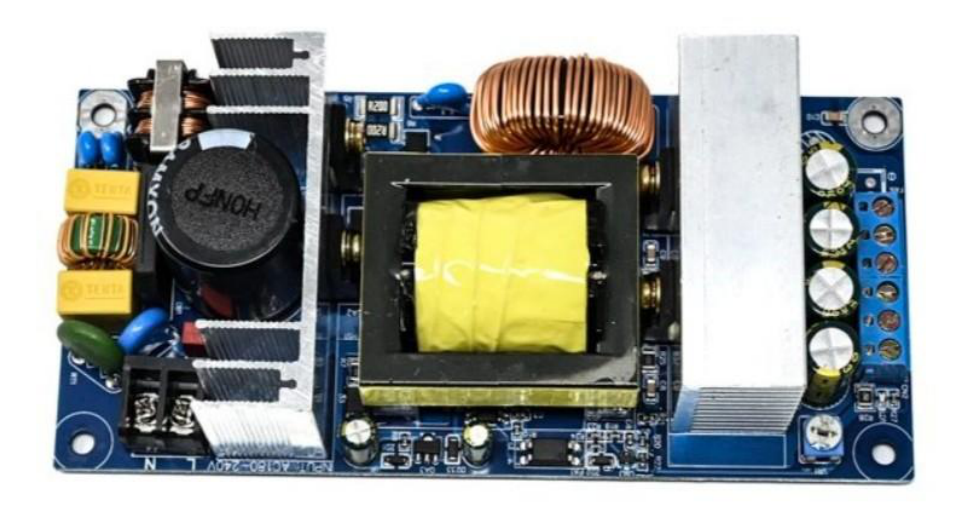
\includegraphics[width=0.46\columnwidth]{fig05a_psu.png}}
\hfil
\subfloat[PZEM-051 power monitor\label{fig:meter}]{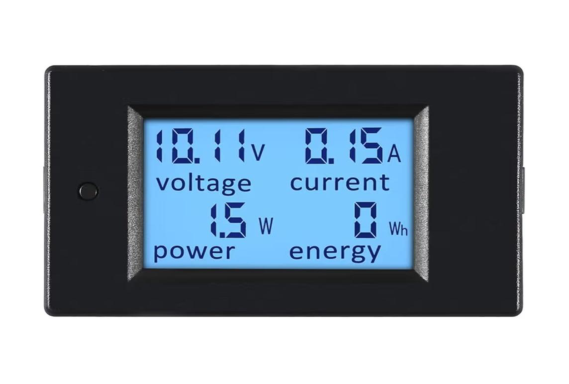
\includegraphics[width=0.46\columnwidth]{fig05b_meter.png}}
\caption{Base-station power and telemetry hardware.}
\end{figure}

\begin{figure}[!t]
\centering
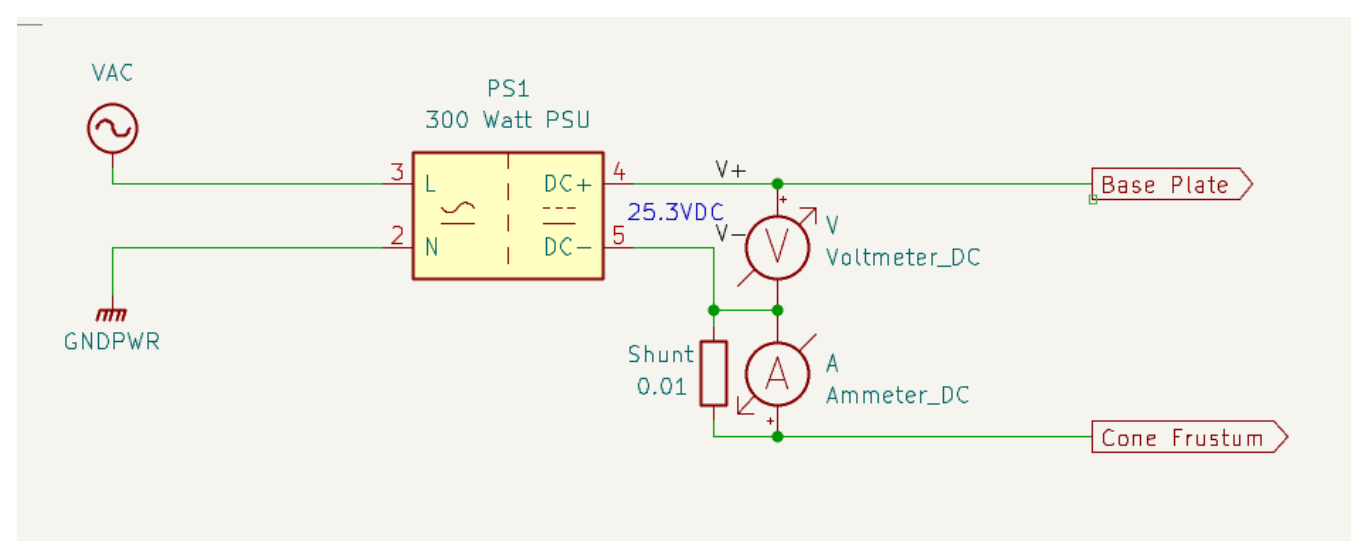
\includegraphics[width=0.92\columnwidth]{fig05c_circuit.png}
\caption{Circuit diagram of the base station, integrating the SMPS, power
monitor, and magnetic charging interface.}
\label{fig:bscircuit}
\end{figure}

\subsection{Airframe}
The airframe uses $250$~mm landing legs to accommodate the magnetic coupling
and LiDAR sensors. The legs are splayed at $23^{\circ}$ to balance bending
stress against an unnecessary rise in the center of gravity (CG); the
vertical CG is established at $255$~mm. Carbon fiber is used as the primary
structural material for its high strength-to-weight ratio, and a modular
architecture allows secure mechanical-fastener attachment of the various
electronic and mechanical subassemblies.

\subsection{Mounts for Electronic Components}
All custom mounts were designed in CAD (SolidWorks/Fusion~360) and
3D-printed in PLA, balancing rigidity, serviceability, and mass.

\subsubsection{Raspberry Pi Casing}
The companion-computer enclosure (Fig.~\ref{fig:pi_case}) protects one of
the primary control units while remaining serviceable. Six evenly
distributed screw holes secure a removable top cover and distribute load
uniformly. Strategically placed side cutouts provide both ventilation for
thermal management and routing for power, GPIO, and peripheral cabling.

\begin{figure}[!t]
\centering
\subfloat[Isometric view]{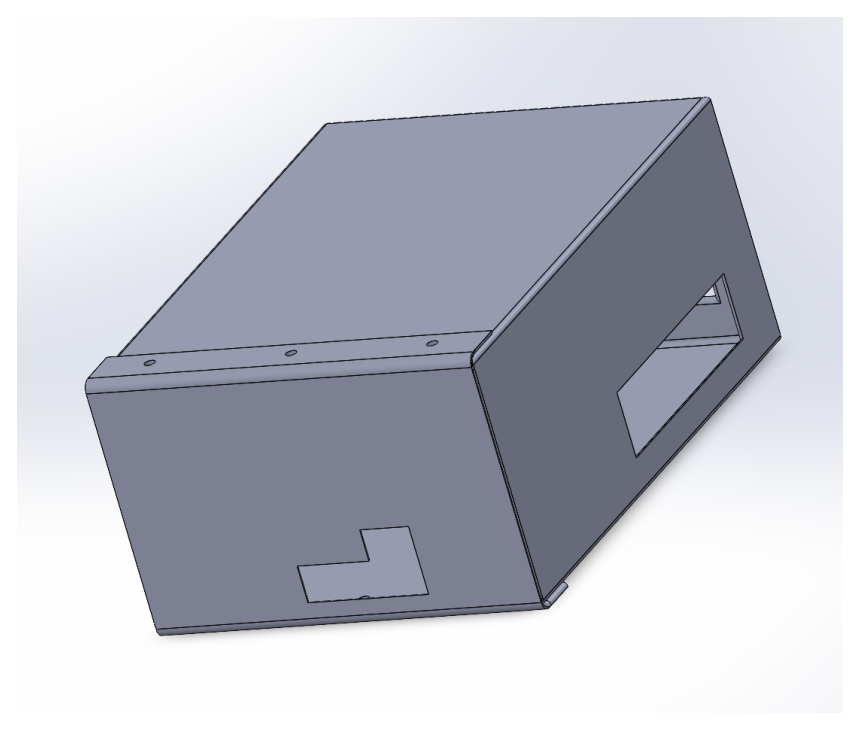
\includegraphics[width=0.46\columnwidth]{fig06a_pi_iso.png}}
\hfil
\subfloat[Individual components]{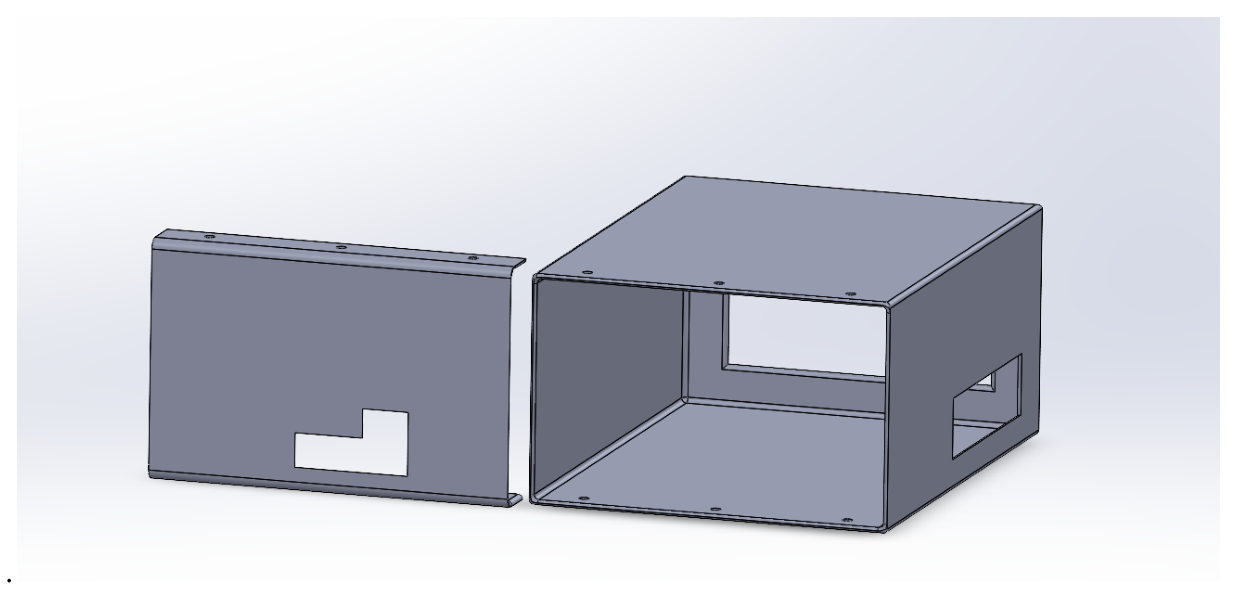
\includegraphics[width=0.48\columnwidth]{fig06b_pi_comp.png}}
\caption{Raspberry Pi enclosure designed for rigidity, ventilation, and
tool-light maintenance.}
\label{fig:pi_case}
\end{figure}

\subsubsection{1D LiDAR Mount}
The 1D LiDAR mount (Figs.~\ref{fig:lidar1d} and~\ref{fig:lidar1d_views})
holds the downward-facing rangefinder in a fixed, ground-normal orientation
for reliable altitude sensing during flight and landing. It is compact to
avoid interference with the crowded lower plate, reuses existing slots for a
secure fit without structural modification, and is stiff enough to resist
the shocks and vibration of landing.

\begin{figure}[!t]
\centering
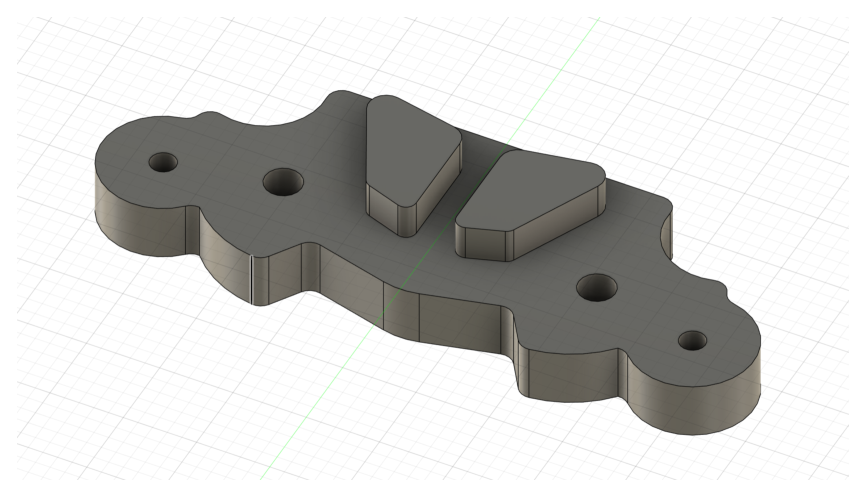
\includegraphics[width=0.62\columnwidth]{fig07_lidar1d.png}
\caption{1D LiDAR mount.}
\label{fig:lidar1d}
\end{figure}

\begin{figure}[!t]
\centering
\subfloat[Front view]{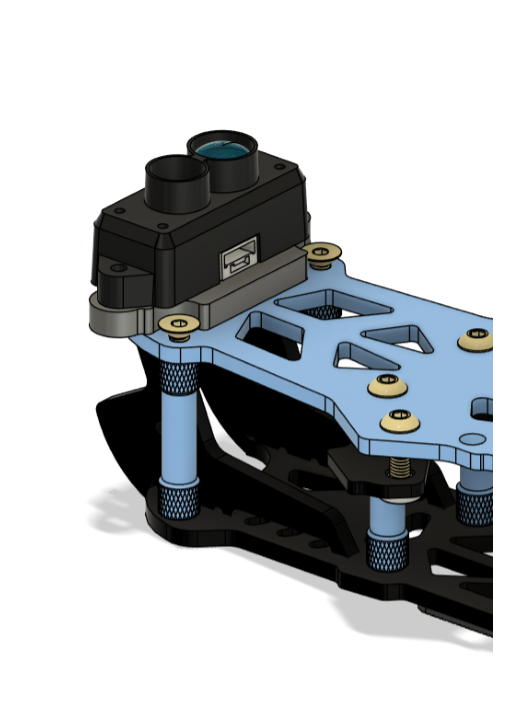
\includegraphics[width=0.40\columnwidth]{fig08a_front.png}}
\hfil
\subfloat[Back view]{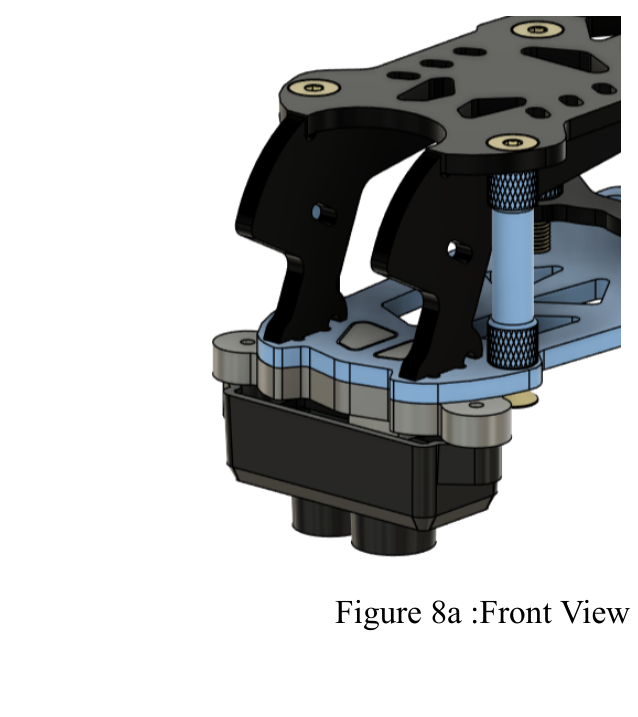
\includegraphics[width=0.40\columnwidth]{fig08b_back.png}}
\caption{1D LiDAR mount, front and back.}
\label{fig:lidar1d_views}
\end{figure}

\subsubsection{Camera Mount}
The camera mount (Fig.~\ref{fig:cam}) is among the most critical structural
components, carrying the global-shutter camera and gimbal. Because looseness
degrades image quality and injects vibration, the design emphasizes rigidity
and precise fit: ten fasteners distribute the combined camera/gimbal load,
and dedicated slots interlock with the gimbal to maintain alignment and
reduce reliance on screws alone.

\begin{figure}[!t]
\centering
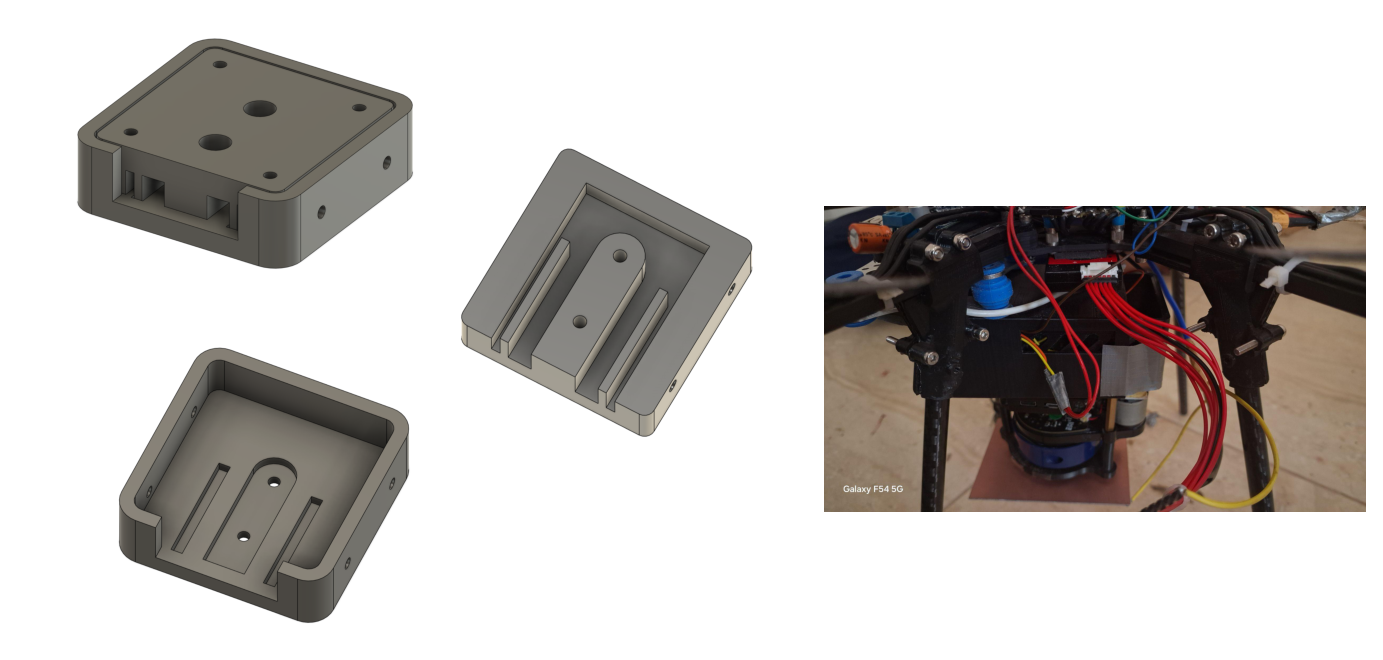
\includegraphics[width=0.92\columnwidth]{fig09_cam.png}
\caption{3D camera mount and its physical implementation.}
\label{fig:cam}
\end{figure}

\subsubsection{2D LiDAR Mount}
The 2D LiDAR mount (Fig.~\ref{fig:lidar2d}) positions the planar scanner
below the main body to lower the CG and improve flight stability, while
preserving an unobstructed $360^{\circ}$ view. The mount is lightweight yet
stiff; it was iterated several times to increase rigidity and suppress
vibration, since excessive vibration corrupts the scan data.

\begin{figure}[!t]
\centering
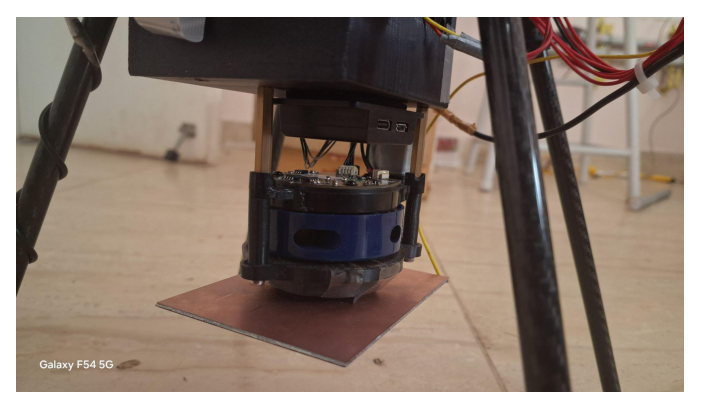
\includegraphics[width=0.72\columnwidth]{fig10_lidar2d.png}
\caption{2D LiDAR mount and its physical implementation.}
\label{fig:lidar2d}
\end{figure}

\subsubsection{Propeller Guards}
The propeller guards (Fig.~\ref{fig:propguard}) protect the relatively
fragile propellers during incidental contact. The design balances low mass
against structural strength, using only the material needed for adequate
rigidity, and achieves a more uniform stress distribution so as to provide
reliable protection without materially degrading aerodynamics.

\begin{figure}[!t]
\centering
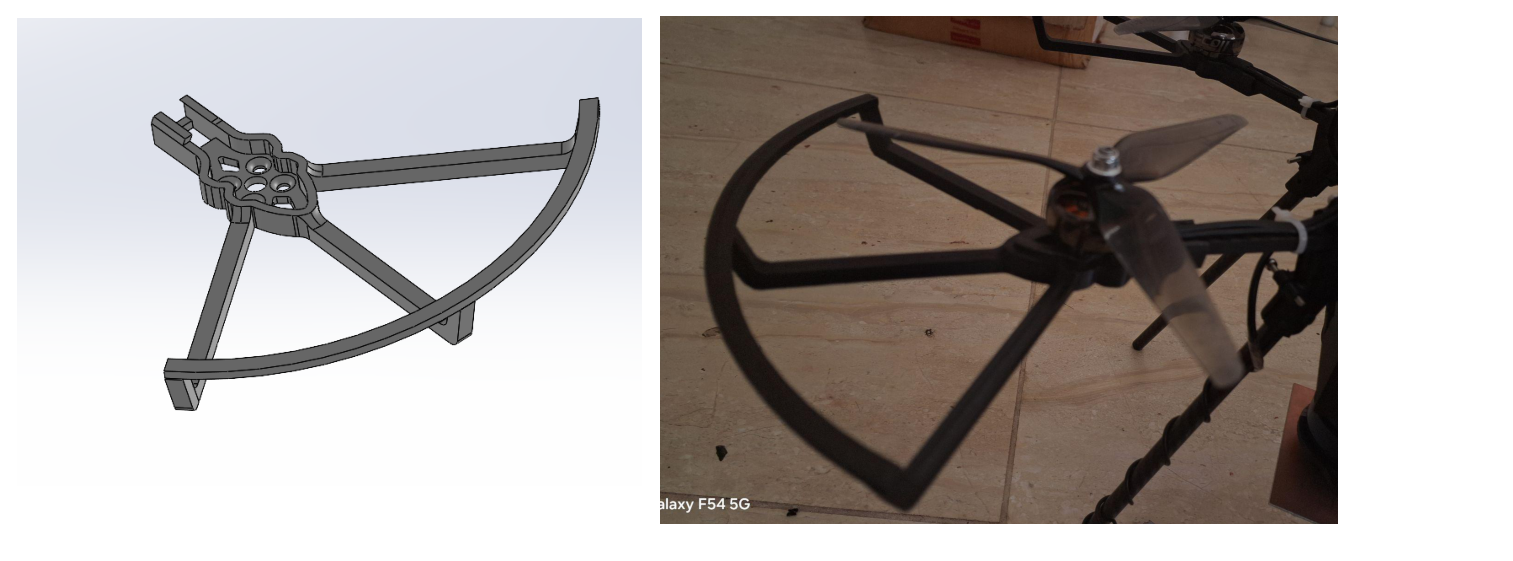
\includegraphics[width=\columnwidth]{fig11_propguard.png}
\caption{Propeller guards and their physical implementation.}
\label{fig:propguard}
\end{figure}

\section{Flight Control}
\label{sec:flight}
The flight stack (ArduPilot/ArduCopter~\cite{ardupilot}) is organized into
three cascaded responsibilities: attitude stabilization via a high-rate
rate loop, altitude hold via sensor-fused barometer and LiDAR, and
GNSS-denied position hold via optical flow.

\subsection{Rate Loop}
The rate loop is the innermost and fastest control layer, directly
responsible for instantaneous angular stabilization. Operating at
$400$\,Hz--$1$\,kHz, it behaves as a high-bandwidth damping system that maps
desired rotation rates to motor commands. It receives target angular rates
(rad/s) from the outer attitude controller and measured gyro rates from the
IMU---sampled at up to $8$\,kHz and filtered through a hardware low-pass
filter and software notch filters to remove vibration harmonics
(Fig.~\ref{fig:pid}).

\begin{figure}[!t]
\centering
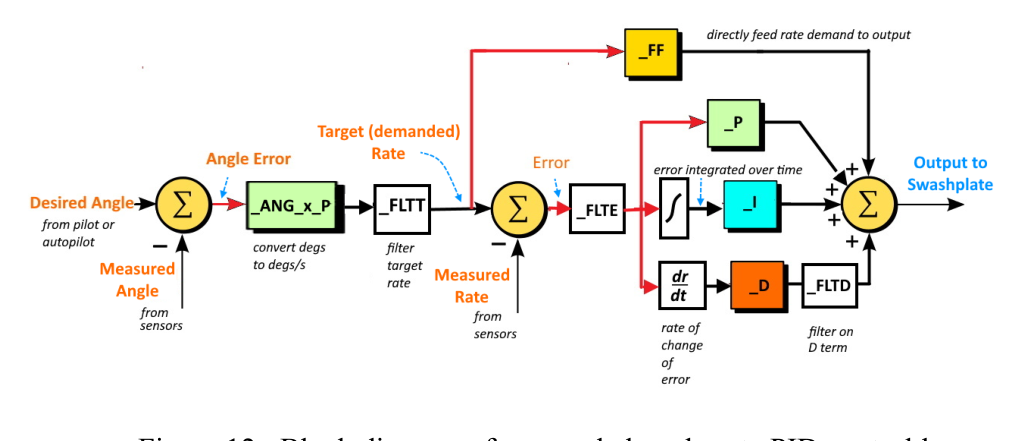
\includegraphics[width=\columnwidth]{fig12_pid.png}
\caption{Block diagram of the cascaded angle--rate PID control loop.}
\label{fig:pid}
\end{figure}

The core feedback law is a PID controller acting on the rate error
$e(t)$:
\begin{equation}
u(t) = K_p\,e(t) + K_i\!\int_0^t\! e(\tau)\,d\tau + K_d\,\frac{d\,e(t)}{dt},
\label{eq:pid}
\end{equation}
where $e$ is the error in the body angular rates (and, for the outer loop,
in roll/pitch/yaw). The proportional term provides immediate correction,
the integral term eliminates steady-state offset (at the risk of windup),
and the derivative term damps oscillations. Three refinements are applied:
\begin{itemize}
\item \emph{Feedforward.} A term $u_{\mathrm{ff}}=r\cdot K_{\mathrm{ff}}$
proportional to the target rate $r$ anticipates the control effort for
commanded motions and reduces phase lag.
\item \emph{Derivative-on-measurement.} The derivative is taken on the gyro
measurement rather than on the error, making the D-term immune to setpoint
steps and eliminating derivative ``kick.''
\item \emph{Dynamic frequency adjustment.} The D-term filter cutoff adapts
to the loop rate, keeping damping consistent across processor loads.
\end{itemize}

\subsection{Altitude Loop}
The altitude loop fuses barometric pressure and downward LiDAR to achieve
centimeter-level hover. The barometer gives absolute altitude but drifts
with weather and is noisy under rotor wash; the LiDAR/ToF sensor gives
accurate relative range (cm resolution) but only within its $\sim\!12$\,m
range and can fail over reflective surfaces. ArduCopter blends the two
through a complementary filter / EKF3: near the ground ($<8$\,m) the LiDAR
dominates for precision; at higher altitude the barometer takes over,
calibrated by LiDAR when available; and weighting is set dynamically from
sensor health and variance.

Control is cascaded into an outer position (altitude) loop and an inner
climb-rate loop. A \emph{dynamic hover throttle} estimator continuously
learns the throttle ($\sim\!40$--$60\%$) required to hold altitude and
updates it during stabilized flight, compensating for changing air density
so that the vehicle holds a constant altitude when commanded.

\subsection{Position Loop (Optical Flow)}
\label{ssec:flow}
Because the vehicle is GNSS-denied, horizontal stabilization uses optical
flow computed onboard. The companion computer performs optical-flow
estimation from the downward camera and supplies velocity and
position-offset data to the flight controller, enabling
centimeter-level position hold indoors and outdoors.

\subsubsection{Principle}
Optical flow measures the apparent motion of brightness patterns between
consecutive frames. Under the brightness-constancy assumption, a pixel of
intensity $I(x,y,t)$ satisfies
\begin{equation}
I_x u + I_y v + I_t = 0,
\label{eq:bcc}
\end{equation}
where $(u,v)$ is the image-plane velocity and $I_x,I_y,I_t$ are the spatial
and temporal gradients. Solving \eqref{eq:bcc} over a feature
neighborhood yields the angular displacement of features, which is converted
to ground-relative velocity using the measured altitude $h$.

\subsubsection{Onboard Implementation}
Frames are converted to grayscale, cropped to the central $60\%$, and
downscaled to reduce load. Corners are detected with the FAST
detector~\cite{rosten2006fast} via \texttt{cv2.goodFeaturesToTrack}, and
tracked across frames with pyramidal Lucas--Kanade~\cite{lucas1981iterative}
(\texttt{cv2.calcOpticalFlowPyrLK}), which handles large displacements
through a multi-scale pyramid. Flow is computed from the old/new corner
correspondences, normalized, and averaged over the frame; a quality metric
derived from the number of good features and the full estimate are
transmitted to ArduPilot via the MAVLink \texttt{OPTICAL\_FLOW} message.
The control integration is
\begin{align}
e_{\mathrm{pos}} &= p_{\mathrm{target}} - p_{\mathrm{flow}},\\
v_{\mathrm{target}} &= \mathrm{PID}_{\mathrm{pos}}(e_{\mathrm{pos}}) + v_{\mathrm{wind}}^{\mathrm{ff}},\\
u_{\mathrm{thr}} &= \mathrm{PID}_{\mathrm{vel}}(v_{\mathrm{target}} - v_{\mathrm{flow}}).
\end{align}

\subsubsection{Estimator Configuration}
To operate without a GPS lock, ArduPilot's estimator was reconfigured to
treat optical flow as the primary horizontal source and the rangefinder as
the vertical source (Table~\ref{tab:ekf}). Robustness parameters were tuned
as follows: \texttt{FLOW\_MIN\_Q} rejects low-quality flow (e.g., in poor
light); \texttt{EK3\_FLOW\_NOISE} and \texttt{EK3\_FLOW\_GATE} trade
responsiveness against jitter; and the velocity/acceleration PIDs were tuned
experimentally from flight logs. EKF3 additionally rejects flow under low
texture, excessive motion blur, or altitude uncertainty $>10\%$, scales
angular to linear velocity using LiDAR/baro altitude, and synchronizes flow
timestamps with the IMU.

\begin{table}[!t]
\centering
\caption{Key Estimator Parameters for GNSS-Denied Operation}
\label{tab:ekf}
\begin{tabular}{lcl}
\toprule
Parameter & Value & Description\\
\midrule
\texttt{AHRS\_EKF\_TYPE} & 3 & Select EKF3 as active estimator\\
\texttt{EK3\_ENABLE} & 1 & Enable EKF3\\
\texttt{EK3\_SRC1\_VELXY} & 5 & Optical flow $\rightarrow$ horizontal vel.\\
\texttt{EK3\_SRC1\_POSZ} & 2 & Rangefinder $\rightarrow$ vertical position\\
\texttt{EK3\_RNG\_USE\_HGT} & en. & Rangefinder for primary height\\
\bottomrule
\end{tabular}
\end{table}

\section{GNSS-Denied Navigation Stack}
\label{sec:nav}
The navigation software is split into a navigation subsystem and an ML
subsystem (Section~\ref{sec:ml}). The navigation stack uses a hierarchical
\emph{two-tier} estimation model that decouples high-frequency local
stabilization from global map consistency.

\subsection{Two-Tier Estimation}
\textbf{Tier 1 --- Local odometry.} The UAV tracks static salient features
(corners and edges) across sequential camera frames. Denoting the camera
pose at time $t$ as a transform $T_t \in SE(3)$, the frame-to-frame
translation $\Delta t$ and rotation $\Delta R$ are fused with IMU data in an
Extended Kalman Filter, yielding a continuous estimate of the local
coordinates $(x,y,z)$ relative to the origin initialized at the
base-station bay.

\textbf{Tier 2 --- Global mapping (SLAM Toolbox).} A lower-rate
($5$--$10$\,Hz) optimization layer ingests 2D-LiDAR scans and the local
odometry to correct drift and construct a globally consistent occupancy
grid~\cite{macenski2020slamtoolbox}. Tracked 2D features are projected into
3D using the camera intrinsics $K$, producing a sparse point-cloud map. When
a target feature (e.g., a layered rock or red-oxide patch) is detected, the
current EKF-derived position is logged and the $(x,y)$ coordinate is appended
to the verification-image metadata.

\subsection{Aerial SLAM}
Autonomous navigation of an unknown environment poses a ``chicken-and-egg''
problem: safe motion needs a map, but accurate mapping needs the robot's
pose. Simultaneous Localization and Mapping (SLAM) resolves this by mapping
the surroundings while localizing the robot within the evolving model.
Whereas ground SLAM need only estimate $x,y,\psi$, aerial SLAM must account
for full 6-DOF motion ($x,y,z$, roll, pitch, yaw).

\subsubsection{Perception and State Estimation}
A UAV requires volumetric perception---lightweight 3D LiDAR or RGB-D
cameras---to avoid overhanging obstacles, in contrast to the single-slice
2D sensing common on ground robots. Lacking wheel odometry, the UAV instead
generates high-rate proprioceptive estimates from the IMU coupled with
optical flow, visual--inertial odometry (VIO), or LiDAR-inertial odometry
(LIO).

\subsubsection{ROS Coordinate-Frame Topology}
Drift is managed through strict frame conventions. The local transform
$\texttt{odom}\!\rightarrow\!\texttt{base\_link}$ is computed by VIO/LIO and
is smooth but drifts over time. The global correction
$\texttt{map}\!\rightarrow\!\texttt{odom}$ is published when the SLAM backend
closes a loop or matches scans to the map; publishing this correction
(rather than snapping \texttt{base\_link} to \texttt{map}) grounds the
vehicle globally while preserving the smooth local transform that the flight
controller depends on. A virtual \texttt{base\_footprint} supports 2.5D
operations such as identifying flat landing zones beneath the drone.

\subsubsection{Spatial Representation and Planning}
Space is discretized with 3D structures (OctoMaps or voxel grids). A 3D cost
map assigns high cost to voxels near structures so that planners such as
A*~\cite{hart1968astar} or RRT* find low-cost trajectories with a volumetric
safety buffer. To track the resulting path, an extension of Pure Pursuit
designates a look-ahead point along the path and continuously adjusts pitch,
roll, yaw, and thrust to chase it.

\subsubsection{Autonomous Frontier Exploration}
To map the arena without a pilot, the vehicle identifies
\emph{frontiers}---the boundaries between mapped free space and unknown
volume~\cite{yamauchi1997frontier}---and selects the next goal by a utility
function that balances frontier size (more map revealed) against distance
(battery economy). It repeatedly pathfinds to new frontiers until the
environment is fully explored.

\subsubsection{Relocalization and Edge Compute}
If the vehicle is moved, rebooted within a known map, or loses tracking, it
relocalizes with 6-DOF Adaptive Monte Carlo Localization
(AMCL)~\cite{fox2001amcl}, scattering pose particles, pruning those
inconsistent with sensor readings, and converging on the true pose---the
classic ``kidnapped robot'' solution lifted into a 6-DOF state space. Because
dense 3D point-cloud processing, pose-graph optimization, and particle
filtering are too heavy---and too latency-sensitive---to offload over Wi-Fi,
SLAM runs entirely onboard. A NVIDIA Jetson Orin Nano is planned for later
rounds, where its GPU accelerates the required vectorized operations.

\section{Perception and Validation Pipeline}
\label{sec:ml}
The vision software is bifurcated into (i) an \emph{onboard} pipeline that
runs visual odometry and lightweight anomaly detection to document candidate
features, and (ii) a \emph{base-station} pipeline that performs heavier,
high-fidelity matching of documented images against the seed images using
scale-invariant features and RANSAC outlier rejection.

\subsection{Photometric Normalization}
Before feature extraction, both seed and verification images undergo
Contrast-Limited Adaptive Histogram Equalization
(CLAHE)~\cite{pizer1987clahe}, mitigating illumination variation, shadows,
and contrast inconsistencies for stable, repeatable detection.

\subsection{Scale-Invariant Feature Extraction}
Validation compares the UAV's documented images against the 3--5 seed images
captured during the seeding task. Because verification images suffer scale,
rotation, and illumination variation, rigid template matching is
insufficient. We therefore use the Scale-Invariant Feature Transform
(SIFT)~\cite{lowe2004sift} at the base station. Although heavier than binary
descriptors such as ORB (preferred onboard for VO), SIFT is far more robust
to the affine distortion expected when a ground feature is imaged from
varying altitude and pitch. SIFT encodes the gradient magnitude and
orientation around each keypoint as a $128$-dimensional descriptor, so that,
e.g., a reflective ice-like patch imaged at $2$\,m matches the seed captured
at $0.5$\,m. All descriptors are $L_2$-normalized for consistent
nearest-neighbor distances.

\subsection{FLANN Matching and Lowe's Ratio Test}
Exhaustive brute-force matching of $128$-D descriptors is inefficient, so we
use the Fast Library for Approximate Nearest Neighbors (FLANN) with a
KD-tree index. Ambiguous matches are filtered with Lowe's ratio test: for a
query keypoint with two nearest neighbors at distances $d_1 \le d_2$, the
match is retained only if
\begin{equation}
d_1 < \gamma\,d_2, \qquad \gamma \in [0.7,\,0.75].
\label{eq:lowe}
\end{equation}
A mutual nearest-neighbor (cross-check) constraint further removes matches
that are not consistent in both directions. The corresponding kernel of the
mask-construction stage is shown in Fig.~\ref{fig:maskcode}.

\begin{figure}[!t]
\centering
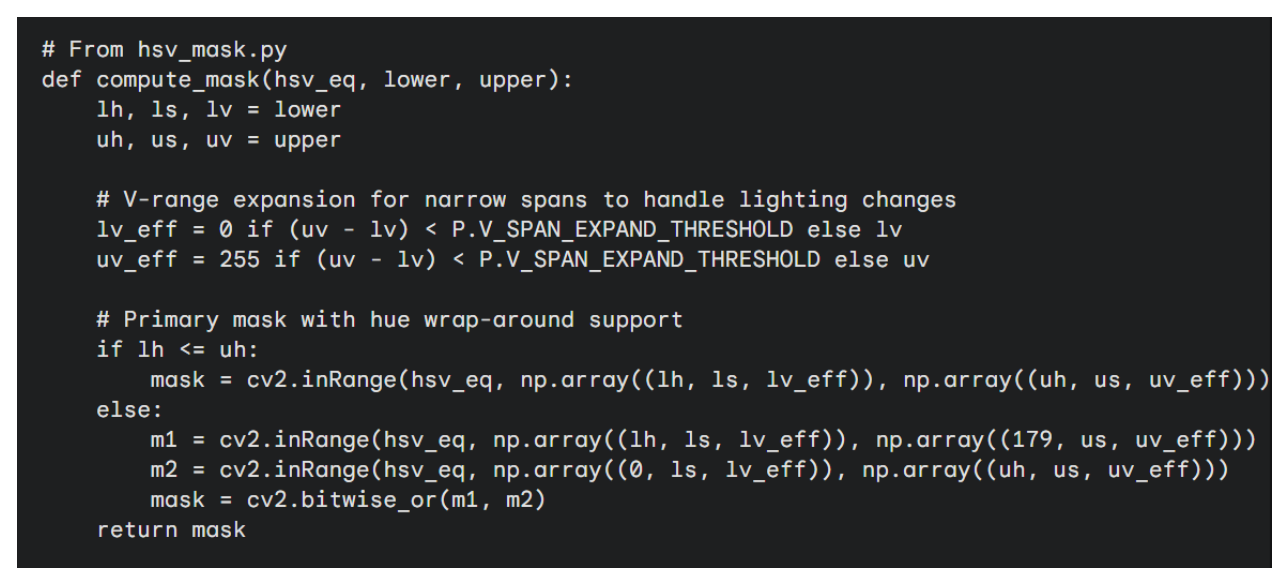
\includegraphics[width=\columnwidth]{fig14_maskcode.png}
\caption{Key code: adaptive HSV mask construction used for base-station
isolation.}
\label{fig:maskcode}
\end{figure}

\subsection{Geometric Verification with RANSAC}
Repetitive arena textures cause residual false positives even after the
ratio test, so detections are geometrically verified with
RANSAC~\cite{fischler1981ransac}. The model is a $3\times3$ homography
$H$ mapping the seed-image plane to the verification-image plane:
\begin{equation}
\begin{bmatrix} x' \\ y' \\ 1 \end{bmatrix}
\sim
H
\begin{bmatrix} x \\ y \\ 1 \end{bmatrix},
\qquad H \in \mathbb{R}^{3\times3}.
\label{eq:homog}
\end{equation}
RANSAC (i) randomly selects $4$ matched pairs to hypothesize $H$;
(ii) projects all matches through $H$ and labels a pair an inlier if the
reprojection error falls below a pixel threshold; and (iii) iterates,
retaining the $H$ with the most inliers. A detection is declared
\emph{valid} when the inlier count exceeds a strict threshold (e.g., $>15$),
the inlier ratio exceeds a minimum, and the reprojection error stays within
limits---jointly enforcing geometric consistency and suppressing false
positives.

\section{Mission State Machine and Precision Docking}
\label{sec:state}
Mission execution on the companion computer is organized as a state machine
governing data flow, the transform hierarchy, and node interactions.

\subsection{State~I: Explorer (Mapping \& Detection)}
In the initial phase the drone builds a map of the unknown environment while
performing seed detection, prioritizing coverage and effective logging
(Fig.~\ref{fig:explorer}). The ODOM node aggregates high-rate inputs from
the camera, the 1D LiDAR (altitude), and camera trigonometry, cross-corrected
against LoRa-module ranging to bound odometry drift; the SLAM node fuses the
corrected odometry with 2D-LiDAR scans into a stored 2D occupancy grid. The
Explorer node acts as the high-level mission commander: it processes 2D-LiDAR
and camera data to find navigable free space and unexplored frontiers,
typically flying at a fixed wall offset and/or following ArUco markers, and
emits dynamic velocity commands (rather than fixed waypoints) to the flight
controller while avoiding obstacles. Concurrently, the ML node embeds the
video feed through a CNN; upon detecting a target on a patch, the Explorer
node centers the feature with a PID controller, tags the image with the
current odometry coordinate, and stores both to the SD card for
post-mission analysis and base-station relay.

\begin{figure}[!t]
\centering
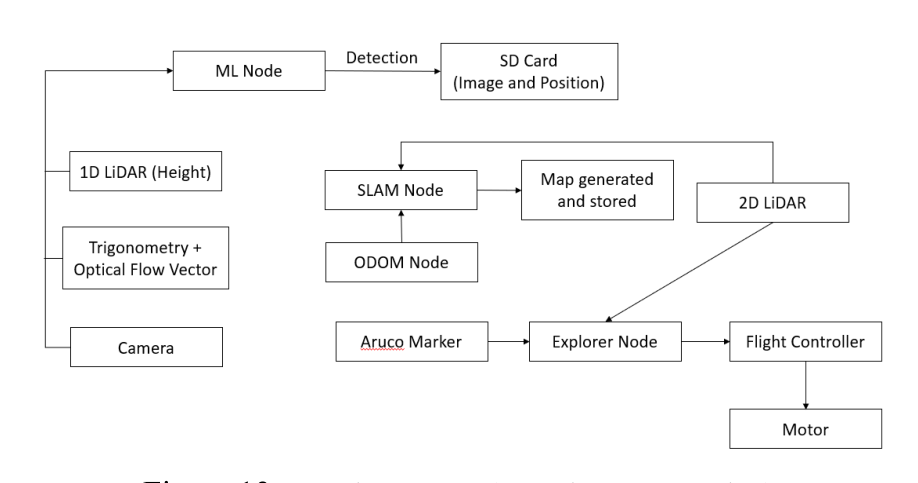
\includegraphics[width=0.86\columnwidth]{fig13a_explorer.png}
\caption{Explorer state: mapping and detection data flow.}
\label{fig:explorer}
\end{figure}

\subsection{State~II: Return-to-Home and Precision Docking}
Once mission objectives are met or a battery threshold is reached, the
system transitions to Return-to-Home, shifting priority from exploration to
precise planning and safe recovery (Fig.~\ref{fig:rth}). The Nav2
stack~\cite{macenski2020nav2} assumes control, replacing the Explorer node,
and uses the static map from State~I to compute a collision-free path back
to the home point with A* over a costmap, running AMCL to avoid dynamic,
previously unmapped obstacles, and issues trajectory velocity commands to
the flight controller.

\begin{figure}[!t]
\centering
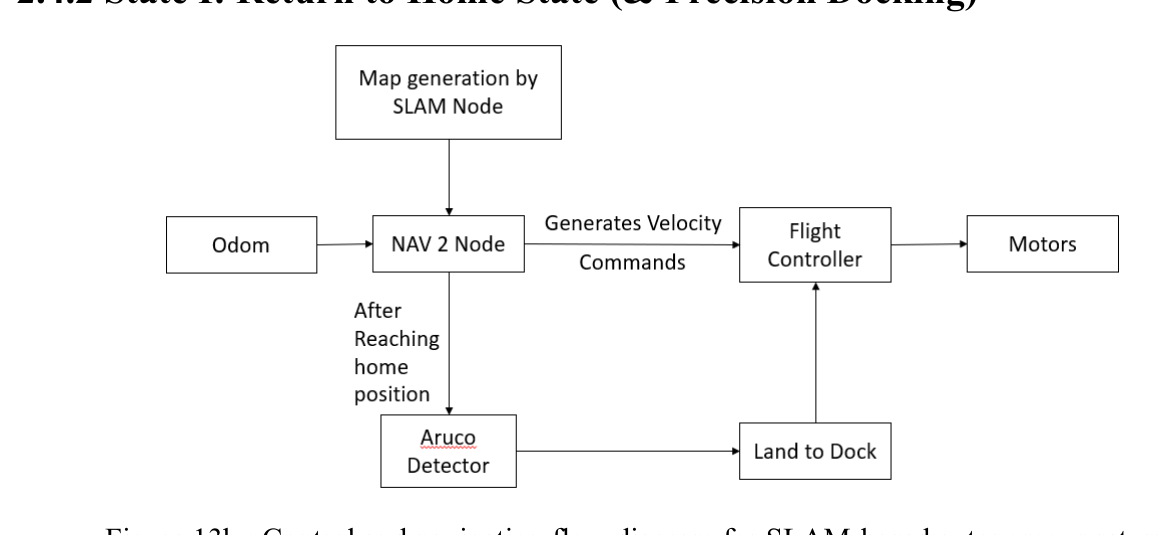
\includegraphics[width=0.92\columnwidth]{fig13b_rth.png}
\caption{Control and navigation flow for SLAM-based autonomous return,
precision docking, and landing using Nav2 and ArUco detection.}
\label{fig:rth}
\end{figure}

\subsubsection{HSV Sampling and Masking}
An adaptive HSV pipeline isolates the base station. Rather than static
thresholds, \texttt{color\_sampler.py} computes a range from a $10$-px-radius
patch, using circular statistics for hue (to handle the $0/179$ wrap-around)
and empirical percentiles for saturation and value (to handle lighting). For
outdoor robustness each frame is bilaterally filtered (edge-preserving) and
CLAHE is applied on the value channel.

\subsubsection{Shape Classification}
Contours extracted from the mask are classified by geometric
metrics---circularity, solidity, aspect ratio, and extent
(Fig.~\ref{fig:quadcode}). Valid base-station shapes include circle, square,
rectangle, ellipse (tilted circle), and trapezoid (tilted
square/rectangle).

\begin{figure}[!t]
\centering
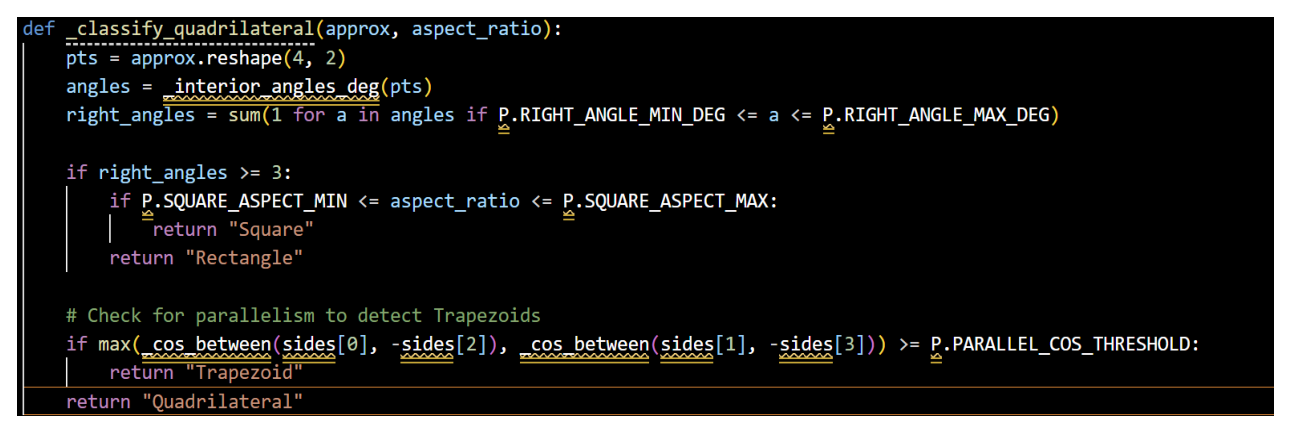
\includegraphics[width=\columnwidth]{fig15_quadcode.png}
\caption{Key code: quadrilateral classification for base-station
identification.}
\label{fig:quadcode}
\end{figure}

\subsubsection{Temporal Stability and 2D-LiDAR Centering}
The vision system performs preliminary identification, after which the 2D
LiDAR centers the vehicle (Figs.~\ref{fig:center} and~\ref{fig:lidarcenter}).
A dedicated node analyzes the LiDAR feed---which traces a circle as the
vehicle enters the frustum---and computes the error between the detected
base-station center and the frame center. The centering workflow is:
(i)~begin descent toward the base station; (ii)~continuously self-center
using HSV masking and visual servoing to estimate $x,y$ offsets and
orientation error; (iii)~simultaneously analyze the LiDAR feed and, once a
circle is detected via the Hough transform, trigger a separate PID
controller that drives the error between the LiDAR-detected circle center and
the vehicle center to zero for touchdown.

\begin{figure}[!t]
\centering
\subfloat[Visual centering on the base station\label{fig:center}]{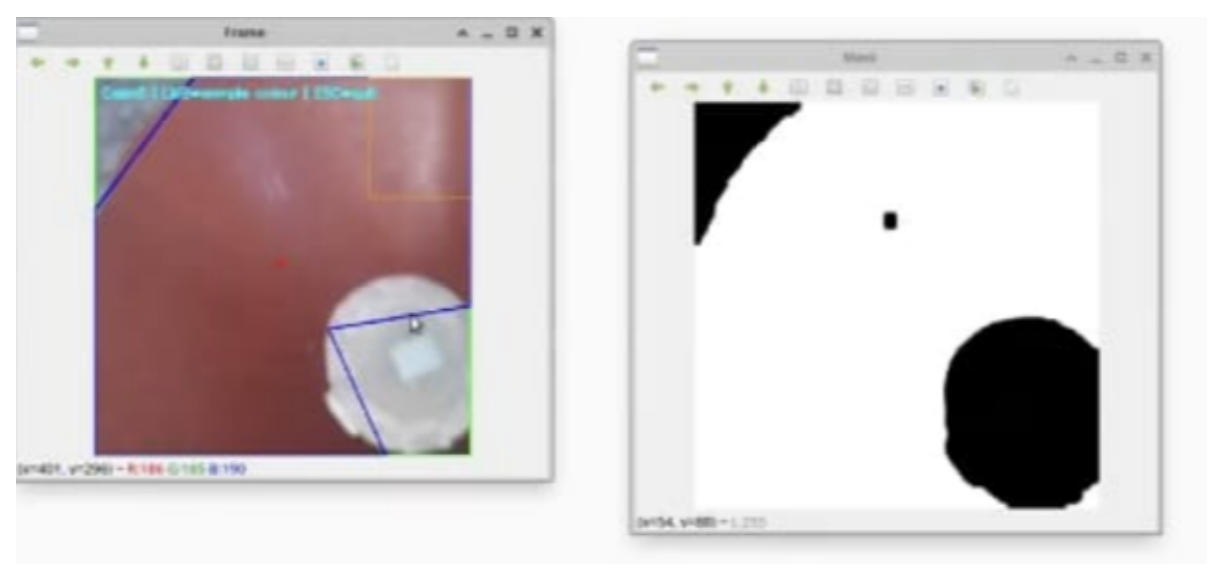
\includegraphics[width=0.52\columnwidth]{fig16_center.png}}
\hfil
\subfloat[2D-LiDAR view during centering\label{fig:lidarcenter}]{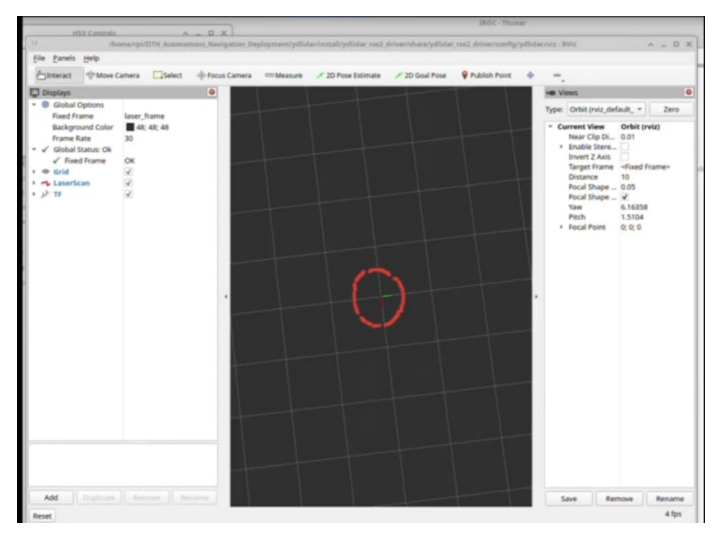
\includegraphics[width=0.40\columnwidth]{fig17_lidarcenter.png}}
\caption{Precision-centering on the base station combining visual servoing
and 2D-LiDAR Hough-circle detection.}
\end{figure}

\section{Hardware Components}
\label{sec:hw}
The hardware was selected for performance, robustness, and integration ease;
the principal items are summarized below and in
Figs.~\ref{fig:frame}--\ref{fig:battery}.

\paragraph{Frame} A GEPRC Mark4 8-inch frame ($367$~mm wheelbase,
Fig.~\ref{fig:frame}) with $6$~mm interlocking carbon arms provides rigidity
and crash resistance while remaining light ($220$~g). It supports both
$30.5\times30.5$~mm and $20\times20$~mm stacks for flexible electronics
integration.

\begin{figure}[!t]
\centering
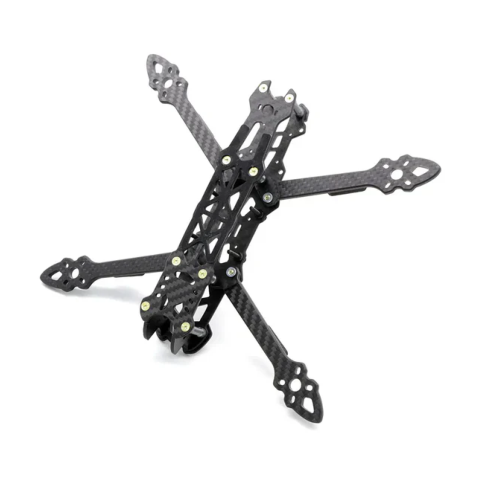
\includegraphics[width=0.55\columnwidth]{fig18_frame.png}
\caption{GEPRC Mark4 8-inch carbon-fiber frame.}
\label{fig:frame}
\end{figure}

\paragraph{Propellers and Motors} Low-pitch $7030$ propellers were chosen
for efficiency, availability, and broad compatibility. The Emax ECO~II
$2807$, $1300$\,KV brushless motors (Fig.~\ref{fig:motor}) deliver
$\sim\!500$~g thrust each at moderate RPM with a low-KV, energy-efficient
profile. With a $4$S pack, hover RPM is $\approx5780$ and full-throttle RPM
is $1300\,\mathrm{KV}\times16.8\,\mathrm{V}=21\,840$, giving a hover throttle
of $\approx26.5\%$ at $\sim\!45\%$ efficiency.

\begin{figure}[!t]
\centering
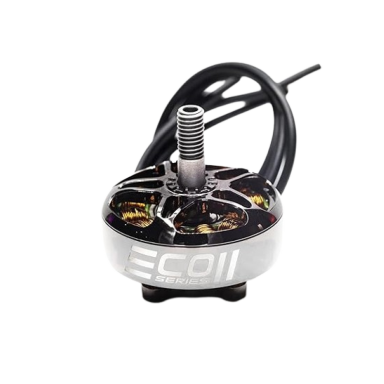
\includegraphics[width=0.45\columnwidth]{fig19_motor.png}
\caption{Emax ECO~II 2807 brushless motor.}
\label{fig:motor}
\end{figure}

\paragraph{Flight Controller} The SpeedyBee F4~V3 (Fig.~\ref{fig:fc}) was
selected for sufficient compute (STM32F405) to sustain high-rate loops,
abundant UART I/O, integrated OSD/barometer/BECs/Blackbox, Bluetooth tuning,
and low cost. Its limitations---F4-class performance, shared OSD/Blackbox
resources, and no onboard magnetometer---are accepted given the
companion-computer-centric architecture; an external magnetometer supplies
heading.

\begin{figure}[!t]
\centering
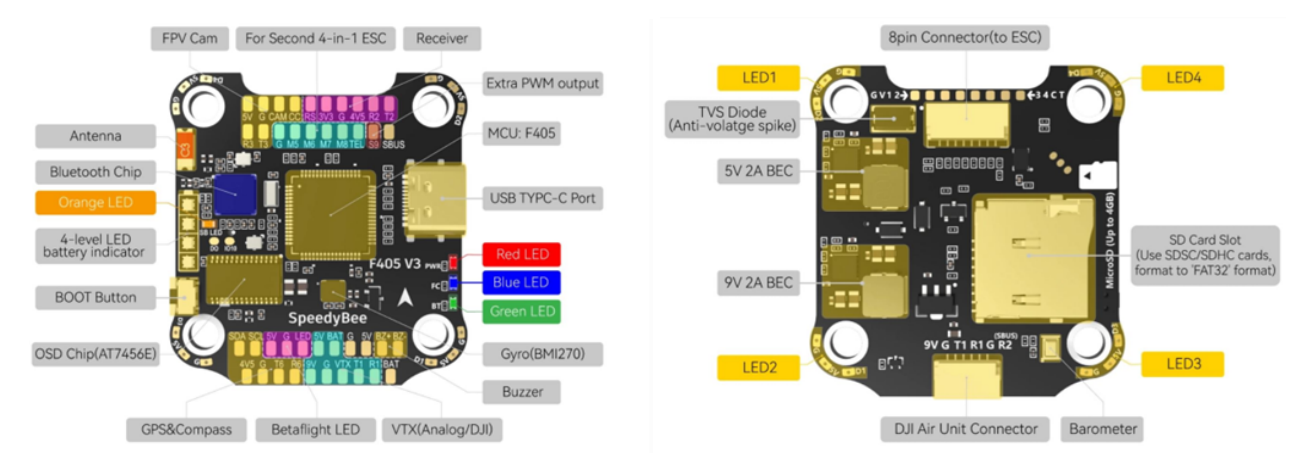
\includegraphics[width=0.9\columnwidth]{fig20_fc.png}
\caption{SpeedyBee F4~V3 flight controller. The FC fuses IMU (and optional
magnetometer/barometer) data to estimate attitude and rates, feeding the
cascaded PID loops and motor mixer.}
\label{fig:fc}
\end{figure}

\paragraph{ESC} A Hobbywing XRotor~G2 4-in-1 ESC ($65$\,A, BLHeli/DShot)
provides a $\sim\!1.5\times$ safety factor over peak motor current draw for
thermal robustness.

\paragraph{Radio} A FlySky FS-i6 transmitter (modded to $10$ channels) with
an FS-A8S receiver (Fig.~\ref{fig:tx}) operates on AFHDS~2A, hopping across
$135$ channels in the $2.408$--$2.475$\,GHz band; the $1.2$~g receiver
supports PPM and i-BUS output.

\begin{figure}[!t]
\centering
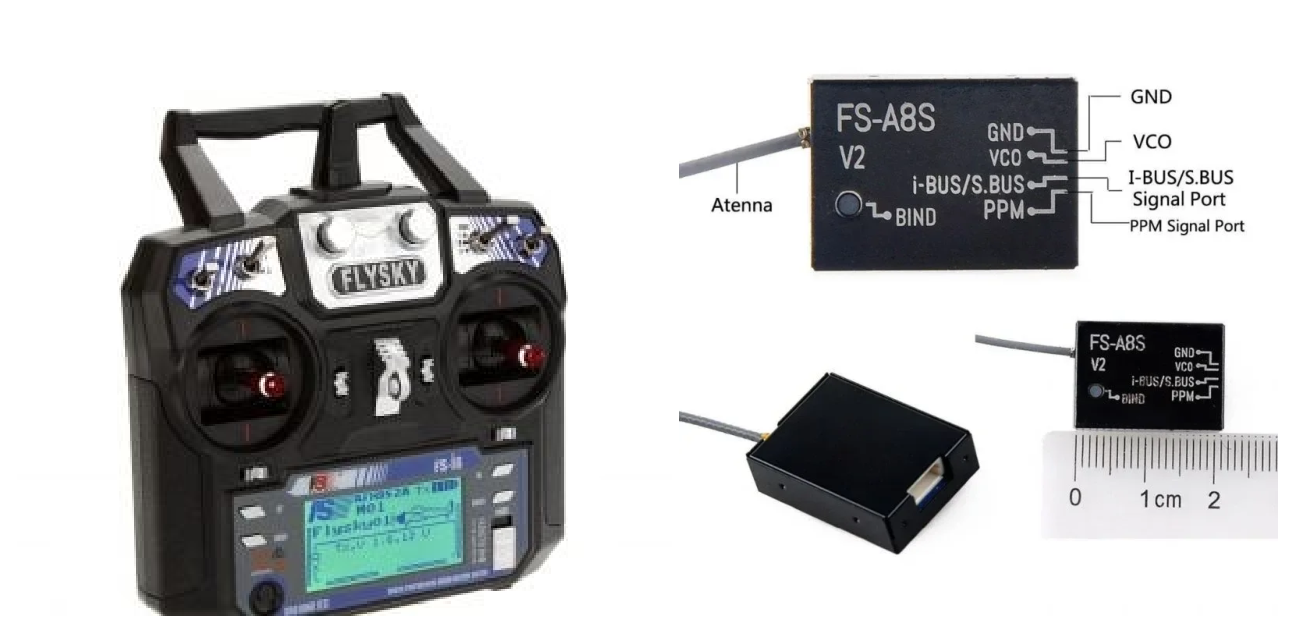
\includegraphics[width=0.9\columnwidth]{fig21_tx.png}
\caption{FlySky FS-i6 transmitter and FS-A8S receiver.}
\label{fig:tx}
\end{figure}

\paragraph{Companion Computer} A Raspberry~Pi~4B
(Fig.~\ref{fig:pi4}; BCM2711 quad-core Cortex-A72, up to $8$\,GB LPDDR4,
Gigabit Ethernet, USB~3.0, MIPI CSI) runs the initial optical-flow pipeline.
For deep-learning inference it is superseded by a NVIDIA Jetson Orin~Nano
(Fig.~\ref{fig:jetson}; Ampere GPU with $32$ Tensor Cores, $\sim\!67$\,TOPS
INT8, $8$\,GB LPDDR5), whose CUDA/TensorRT acceleration makes CNN inference
real-time---infeasible on a CPU-only board.

\begin{figure}[!t]
\centering
\subfloat[Raspberry Pi 4B companion computer\label{fig:pi4}]{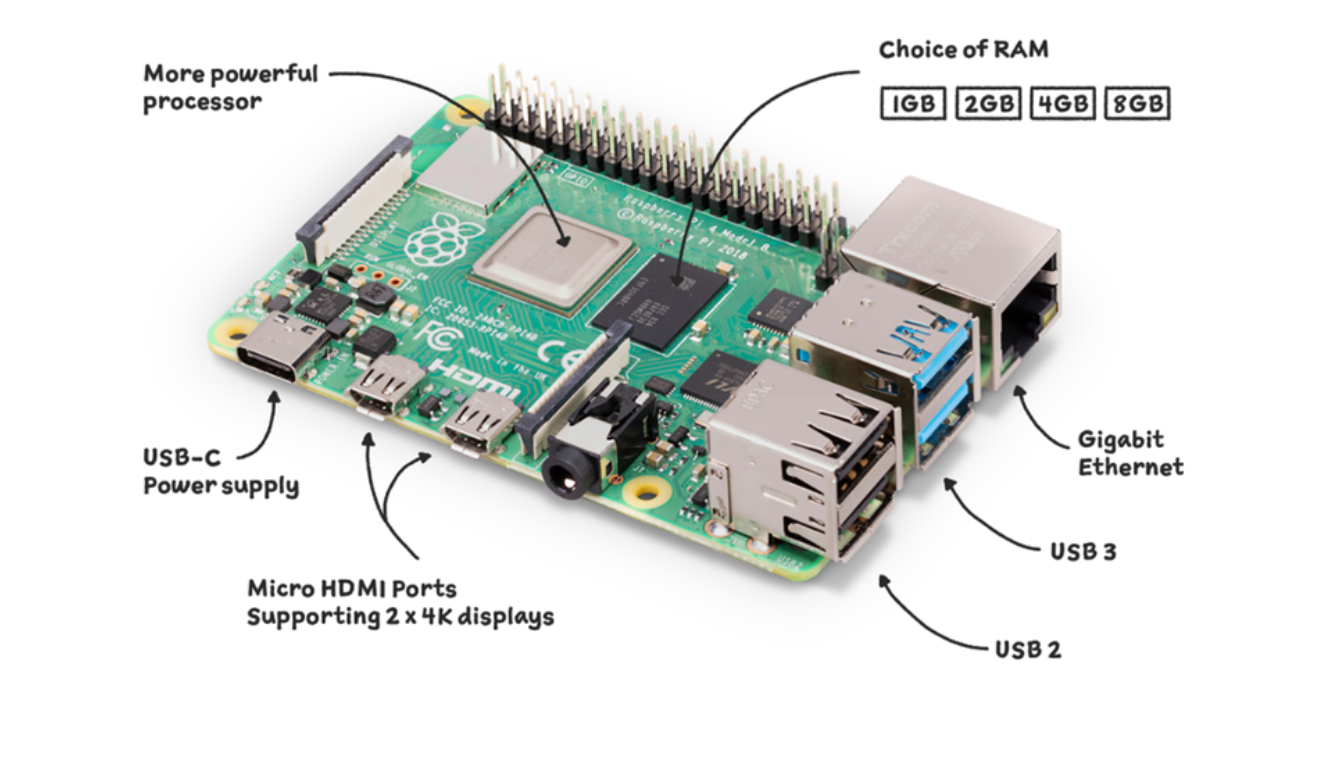
\includegraphics[width=0.62\columnwidth]{fig22_pi4.png}}\\
\subfloat[NVIDIA Jetson Orin Nano (planned upgrade)\label{fig:jetson}]{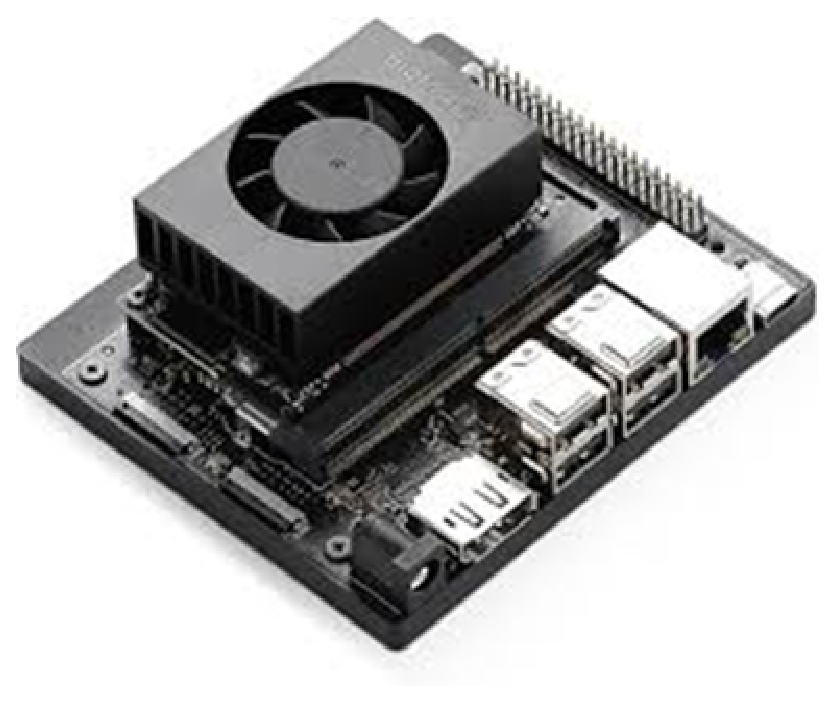
\includegraphics[width=0.6\columnwidth]{fig23_jetson.png}}
\caption{Onboard compute. CPU-only optical flow runs on the Pi; GPU-bound
CNN inference is offloaded to the Jetson.}
\end{figure}

\paragraph{Optical-Flow Camera} An Arducam global-shutter OV9281
(Fig.~\ref{fig:ofcam}) supplies the downward image stream. Flow is computed
from consecutive frames (sparse Lucas--Kanade or dense
Farneb\"ack~\cite{farneback2003two}) under the brightness-constancy model of
\eqref{eq:bcc}, with pixel displacement converted to velocity via camera
calibration and altitude.

\begin{figure}[!t]
\centering
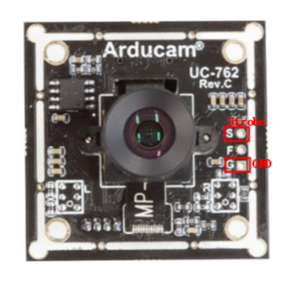
\includegraphics[width=0.4\columnwidth]{fig24_ofcam.png}
\caption{Arducam global-shutter OV9281 optical-flow camera.}
\label{fig:ofcam}
\end{figure}

\paragraph{Rangefinders} A Benewake TFmini-S 1D LiDAR
(Fig.~\ref{fig:tfmini}; $0.1$--$12$\,m, $\pm6$~cm to $6$\,m, up to
$1000$\,Hz, $2^{\circ}$ FoV, $5$~g) provides altitude, and a YDLIDAR~X2 2D
scanner (Fig.~\ref{fig:ydlidar}; $360^{\circ}$, $0.12$--$8$\,m, $5$--$8$\,Hz
scan) provides planar perception for SLAM and obstacle avoidance.

\begin{figure}[!t]
\centering
\subfloat[Benewake TFmini-S (1D)\label{fig:tfmini}]{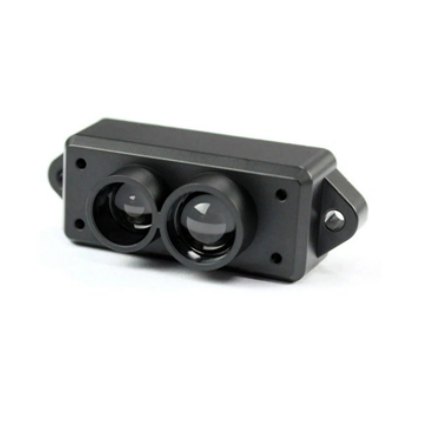
\includegraphics[width=0.42\columnwidth]{fig25_tfmini.png}}
\hfil
\subfloat[YDLIDAR X2 (2D)\label{fig:ydlidar}]{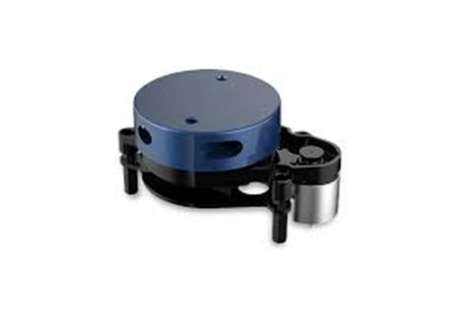
\includegraphics[width=0.42\columnwidth]{fig26_ydlidar.png}}
\caption{LiDAR rangefinders for altitude and planar perception.}
\end{figure}

\paragraph{Power Electronics} An XY-3606 buck converter
(Fig.~\ref{fig:buck}; $9$--$36$\,V in, $5.2$\,V out, up to $30$\,W,
$\le95\%$ efficiency) supplies the avionics rail, protected by a $6$S BMS
(Fig.~\ref{fig:bms}; balance, over-charge/discharge protection, IP65/67).
A $6$S LiPo (Fig.~\ref{fig:battery}) powers the propulsion system.

\begin{figure}[!t]
\centering
\subfloat[XY-3606 buck converter\label{fig:buck}]{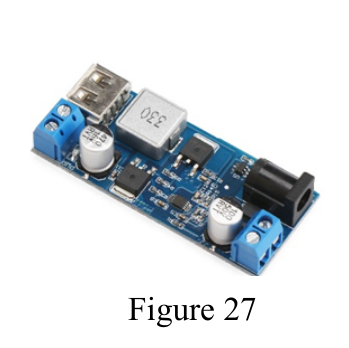
\includegraphics[width=0.30\columnwidth]{fig27_buck.png}}
\hfil
\subfloat[6S BMS\label{fig:bms}]{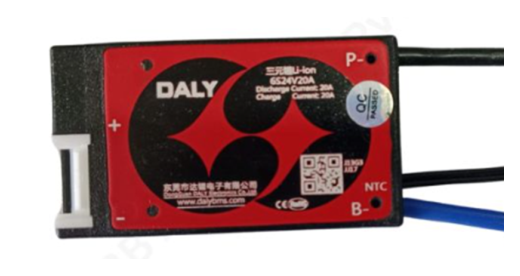
\includegraphics[width=0.30\columnwidth]{fig28_bms.png}}
\hfil
\subfloat[6S LiPo battery\label{fig:battery}]{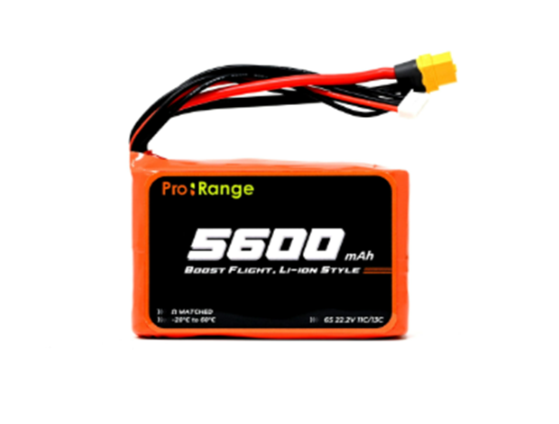
\includegraphics[width=0.30\columnwidth]{fig29_battery.png}}
\caption{Onboard power electronics and energy storage.}
\end{figure}

\section{System and Power Budget}
\label{sec:budget}
The overall system specification is summarized in
Table~\ref{tab:spec}. The power budget is dominated by propulsion. Summing
the flight controller ($12$\,W), four motors ($4\times100=400$\,W), and the
companion computer ($27$\,W) gives a total draw of $\approx439$\,W. At a
nominal $22.2$\,V this is an average current of
$439/22.2 \approx 19.77$\,A. With a $5600$\,mAh, $13$C pack the maximum
discharge current is $13\times5.6 = 72.8$\,A, a safety factor of
$72.8/19.77 \approx 3.68$. The expected endurance is
$5.6\,\mathrm{Ah}/19.77\,\mathrm{A} \approx 0.283$\,h, i.e.\ about
$16$~minutes of flight per charge.

\begin{table}[!t]
\centering
\caption{System Specification}
\label{tab:spec}
\begin{tabular}{ll}
\toprule
Parameter & Specification\\
\midrule
Overall mass & $1900$\,g\\
Overall dimensions & $450\times500\times350$\,mm\\
Power requirement & $300$--$500$\,W\\
Flight time per charge & $10$--$15$\,min\\
Propellers & $4\times7030$\\
Key features & GNSS-denied navigation, image\\
 & recognition, auto-docking\\
\bottomrule
\end{tabular}
\end{table}

\section{Emergency-Response System}
\label{sec:safety}
Safety is enforced at several layers. An emergency call-off provides both a
hardware kill switch (via an ARM switch) and a manual-override command (via
the MAVLink override feature): the former cuts motor power in
$<200$\,ms, while the latter hands full authority to the pilot in
stabilize mode. Automatic failsafes cover battery, radio, and EKF
position-estimate failure. Obstacle avoidance (in progress) uses the 2D
LiDAR to maintain standoff from obstacles, with the camera providing
supplementary detection.

\section{Novelty}
\label{sec:novelty}
The principal novelty is software-centric. The system is built on ROS~2,
decomposing sensing, localization, mapping, planning, and mission management
into modular nodes with well-defined interfaces and reliable inter-node
communication, which enables asynchronous sensor processing and scalable,
testable development. Environment understanding uses a 2D-LiDAR sensing
pipeline that converts raw scans into a planar occupancy representation and,
from it, local and global costmaps in which obstacles are inflated by the
vehicle footprint and safety margins and continuously updated as new
obstacles are observed. Localization uses AMCL on the generated map for
probabilistic robustness and recovery from uncertainty, while the Ceres
Solver performs nonlinear optimization to reduce accumulated drift and
improve spatial coherence. Path planning uses A* over the global costmap for
collision-free, cost-efficient trajectories, with a locally updated costmap
for short-horizon adjustments. Together, ROS~2 modularity, 2D-LiDAR costmap
generation, AMCL localization, Ceres-based optimization, and A* planning form
a robust, computationally efficient navigation stack tailored to GNSS-denied
autonomous exploration.

\section{Conclusion}
\label{sec:concl}
We presented ASCEND, an autonomous quadrotor--base-station system for
GNSS-denied exploration, mapping, feature identification, and precision
self-recovery. The design integrates a self-aligning frustum docking
platform with automatic magnetic charging, a cascaded ArduPilot flight stack
reconfigured for optical-flow and rangefinder-driven station keeping, a
two-tier estimation and 2D-LiDAR SLAM navigation stack with frontier
exploration and AMCL relocalization, and a SIFT/FLANN/RANSAC validation
pipeline that matches documented features against seed imagery. The complete
mechanical, electrical, and software subsystems, together with the power and
mass budget and a layered emergency-response architecture, yield a coherent
and reproducible platform. Future work targets full onboard GPU acceleration
on the Jetson Orin Nano, completion of LiDAR-based obstacle avoidance, and
field validation of the end-to-end autonomous mission.

\section*{Acknowledgment}
The authors thank Team Robotech, NITK, and the organizers of the ISRO
Robotics Challenge--Unmanned (IRoC-U) 2026.

\bibliographystyle{IEEEtran}
\bibliography{refs}

\end{document}
